\chapter{Introduction}
\label{chapter:introduction}

\section{Context and Motivation}

The IT industry and the penetration of IT services into the life of most people has entered a new era. The number of devices connected to the internet has been growing steadily.  Cisco estimated that by 2008 the number of internet-connected devices had exceeded the number of people in the world and that by 2011 the internet usage of 20 typical households was generating more internet traffic than the world's entire  internet use in 2008 \cite{evans2008-iotinfo}. Partly due to this network capacity, we are witnessing a parallel growth in data, driven by more affordable storage systems and  new applications of the internet including mobile applications, IoT, social media, and smart cities.  This combination of data and connectivity has resulted in so-called "digital transformation" in many industries, leading to a huge ecosystem of software applications, from business analytics of customer behaviour to mobile apps that can allow a farmer to monitor the climatic and ground conditions in their fields in real time through local sensor systems. These new applications rely on being internet-connected, which results in constantly increasing demand for private and "cloud" data centre capacity.  This is why large Tech companies and major enterprises are continuously expanding their computing capabilities. 

Currently, data centres consume a substantial amount of energy and are thought to produce more greenhouse gas emissions than the entire aviation sector. In 2013, data centres in the U.S. alone consumed an estimated 91 billion kWh of electricity, and this is expected to rise to 140 billion kWh recent survey of data centre managers showed that energy efficiency is seen as their single biggest challenge \cite{cainc2016-ausdcenergy}. This is particularly important for colocation and managed service data centre providers who are based within or close to large cities where grid power availability is limited.

So, can the data centre community evolve to cope with this ever-increasing demand and support the world's relentless digital transformation? We cannot be sure, but it is clear that the challenges that it poses are widely understood.  A large number of industrial, governmental and academic research programmes \cite{loken2010-scinet, bahsoon2010-cloudpower, greengrid2011-dcefficiency, dc4cities2014_dcmetrics,ida2015-gdcip} have been investigating and continue to explore topics that can help, from new cooling technologies to more energy-efficient servers and building designs in the physical domain, from runtime workload consolidation to energy consumption monitoring in the software domain and even economic models for balancing system quality properties and power consumption from cross-disciplinary research. However, the software architecture community has been slower to recognise their potential contribution and to mobilise to meet this challenge. Addressing energy efficiency at the architecture level is still far from being mainstream. Can we continue designing systems without any consideration of their energy and power efficiency and let others worry about running them in an energy-efficient way? Should energy efficiency be a bolt-on system property or a quality attribute that is addressed at design time?

We believe that software architects may not be prioritising energy efficiency for a number of reasons.

Firstly, we currently have very little understanding of the impact of design decisions on energy efficiency or an understanding of how it affects other system qualities such as user experience, reliability, and performance.  Without this knowledge, it is difficult to perform trade-off analysis to understand the benefit or cost of improving energy efficiency. Minor changes to the system design could yield substantial benefits, such as avoiding unnecessary component redundancy or eliminating low-priority housekeeping tasks that prevent equipment from entering lower-power states. However, a lack of relevant design tools and frameworks mean that it is still difficult to understand the energy characteristics of software at an architectural level, let alone understand or test the energy implications of design decisions. 

Second, in order to achieve the next order of magnitude in energy efficiency, we need to think outside traditional design boundaries. This will require people from different specialisations and departments to prioritise energy efficiency as a design goal and to work together. This can often be difficult to achieve, given current organisational governance structures, with different teams sometimes having competing objectives, not to mention human dynamics and political barriers.

Finally, with the exception of mobile applications, where battery life is a visible reminder of the need for energy efficiency, energy rarely features as a high priority requirement or concern for system acquirers or end-users. On one hand, there is the problem of split incentives where operators of systems (e.g. administrators or data centre managers) do not pay the energy bill (which usually comes from the facilities budget). This means that they would see very little return from any savings made from energy efficiency. On the other hand, while energy costs can be anywhere from 25\% to 60\% of total data centre operating cost \cite{techuk2013-dcpower}, this is often a relatively small percentage of an organisation's overall spending. So, when cost savings are required, it may be easier to achieve them by reducing cost in other areas.

We believe that this situation can be addressed by creating tools and guidance which is aimed specifically at software architects and system stakeholders, to allow them to understand the energy efficiency implications of architectural design decisions.  The work reported in this thesis is a first step on the road to provide this.

\section{Objectives and Research Questions}

The objective of this research is to improve the assistance available to software architects to help them understand the impact of their work on the energy efficiency of the systems that they design.  This process started in the area of architectural description languages (ADLs) because the unambiguous description of the architecture that they provide offered the potential to provide the architect with visibility of the energy implications of their design decisions.

To reach our objective, this work aims to answer four specific research questions, namely:
\nopagebreak
\begin{description}
\item [RQ1] What architecture description languages exist and can they be used to reason about the energy properties of a system?
\item [RQ2] How can architects prioritise energy efficiency as an architectural concern?
\item [RQ3] What design guidelines can we provide to assist architects to improve the energy efficiency of their systems?
\item [RQ4] How can we make architects aware of the runtime energy characteristics of their systems?
\end{description}

Answering these questions has involved the investigation of the use of ADLs for large-scale architectural description, the identification of practical advice for how architects can focus attention on critical topics (such as energy efficiency), the identification of design principles to guide energy-efficient architectures, and the creation of a practical approach for estimating the energy usage of request processing in distributed applications.

\section{Research Methodology}

The research reported in this thesis comprises four areas of investigation, aligned with the four research questions defined above.  Each area of investigation has utilised different combinations of research techniques, which are outlined below.  Fuller discussion of the research methdology for each piece of work is provided in the relevant chapters of the thesis.

\subsection{Architectural Description Languages Investigation}

The ADL investigation work began with a systematic literature review \cite{kitchenham2007-slr}, which was presented in \sref{sec:adl-lit-review}, with the goal of systematically identifying, analysing and understanding the work that had been done to date in creating and applying architectural description languages.  

The second stage of this research was to undertake a practical exercise to apply an ADL from the research results to the description of a large industrial system to understand how practical and effective this would be.

This research enabled us to answer research question RQ1.

\subsection{Study of Prioritising Architectural Effort}

Our study of architectural effort prioritisation began with a narrative literature review to survey the state of research in this area \cite{baumeister1997-narrativereviews}, which is described in \sref{section:litreview-prioritisation}.  The literature review did not identify a satisfactory approach to the problem of prioritising architectural effort, so we undertook the process of creating one.  This a was a four-stage process involving surveys, model building and validation.  Full details are provided in \cref{chapter:prioritisation}, but in summary, the four stages of research were:
\nopagebreak
\begin{description}
	\item [Stage 1] gathering primary data using semi-structured interviews with practitioners, using a written introduction to the question we wanted to answer and then some specific questions to illustrate our area of interest. 
	\item [Stage 2] analysis of the primary data and creation of a preliminary model through a simple application of Grounded Theory \cite{charmaz2006-groundedtheory}.
	\item [Stage 3] validation of the preliminary model via a structured online questionnaire \cite{gillham2000-questionnaire}, completed by practitioners in relevant architecture roles (primarily software, solution and enterprise architects).
	\item [Stage 4] analysis of the validation data and refinement of the preliminary model into a final, validated model.
\end{description}

To ensure practitioner involvement in the research, we used the LinkedIn and Twitter social media networks to publicise and engage with architecture practitioners and to report preliminary results.

The result of this research was a validated model to guide the prioritisation of architectural effort, which allowed us to answer research question RQ2.

\subsection{Development of Energy Efficiency Design Principles}

This aspect of the research was undertaken to answer research question RQ3 by attempting to identify energy efficiency related design guidance for practicing software architects.

The work began with a narrative literature review to survey the state of research in this area, described in section \sref{section:litreview-energyguidance}, which identified some useful ideas in the research literature, but relatively little design guidance relevant to the software architecture practitioner.

To identify some initial design guidance we decided to study an industrial situation that had been successful in reducing energy consumption and found a case study from a major internet firm that had managed to reduce energy consumption considerably \cite{ebay2013-digitalefficiency}.  We analysed this scenario and synthesised and captured key principles from it.

This enabled us to answer research question RQ3.

\subsection{Design and Implementation of Application Energy Monitoring}

This section of the research aimed to answer research question RQ4 through the design and implementation of a proof-of-concept implementation of a technical solution to provide architects with visibility of the energy consumption of their systems.

The work began with a narrative literature review to survey the state of research in this area, reported in \sref{sec:litreviewenergy}.  This exercise discovered that some application energy measurement systems have been designed and reported in the literature, but most are not available for general use and the solutions proposed all had some significant limitations when their application to industrial systems was considered.



This work designed a novel approach to capturing representative energy usage for application execution scenarios, that allocates estimated server energy usage to the applications running on that server, rather than trying to calculate an absolute energy consumption for each.  The approach was implemented using modern mainstream technology (such as Linux, Docker and Java) and then validated using a set of practical, realistic tests, to validate its internal consistency and external correctness with respect to its runtime environment.

The design is presented in a technology independent way in \cref{chapter:monitoring}, the concrete implementation is described in \cref{chapter:implementation} and the validation process is described in \cref{chapter:validation}.

A fuller description of the research methodology for the entire exercise, described in the three chapters, is presented in \sref{section:apollo-research-method} in \cref{chapter:monitoring}.

The competion of this work enabled us to answer research question RQ4.

\section{Contribution}

The research described in this thesis has contributed elements to software architecture research and energy efficiency research and in particular, has contributed to bringing the two closer together.
\pagebreak
The specific research contributions in this thesis are as follows: \nopagebreak
\begin{enumerate}
	\item \textbf{A comprehensive systematic survey of architecture description languages}.  This literature review surveyed all ADLs created from 1991 to 2015, reviewing 135 potential languages, with 51 of them being confirmed as architectural description languages, according to our criteria.  A detailed characteristation of the languages and the field were produced from this analysis.
	\item \textbf{A case study of practical ADL use at scale in industry}.  Having surveyed the ADLs, we considered how to apply them to a real problem for a real stakeholder for a large industrial system.  This experience led to the academic ADLs being abandoned and a simple, lightweight, specialised notation to describe the architectural style used in the system being used instead.  A set of lessons learned and constructive suggestions for future ADL research were derived from the experience.
	\item \textbf{A model for architectural effort prioritisation}.  We interviewed expert practitioners and created a model for effort prioritisation based on common approaches that they (unknowingly) shared.  This model was then validated and refined using the results of a survey of 84 software architecture practitioners from across the world.
	\item \textbf{Principles for energy-efficient architectural design}.  Having found no energy specific architecture principles and relatively few generally applicable energy efficiency tactics in the literature, we identified a small set of principles from a successful industrial case study that reduced energy consumption for application services.
	\item \textbf{A system for allocating energy to application scenarios}.  Our literature review revealed that a number of application energy estimation systems had been proposed and prototyped.  However, all of these systems measure the energy consumption of operating system processes, which makes the information of limited immediate value to the application architect.  Our contribution has been to design and create a proof-of-concept implementation of a system which estimates the energy consumption of execution scenarios through the application (using application tracing), so providing the architect with significantly more insight into the effect of their architectural decisions. As far as we know, this scenario based energy usage calculation has not been attempted before in prior research.
	\item \textbf{Open source implementation of Apollo}.  The proof-of-concept implemenation of the system for allocating energy to application scenarios is available as open source software, under an Apache license, from the well known Github source repository site at \texttt{http://github.com/eoinwoods/apolloenergy}.
\end{enumerate}

Much of the work reported here has been previously published in conference proceedings and journals. The publications arising from this work are listed below: \nopagebreak
\begin{description}
	\item Woods, Eoin, and Bashroush, Rabih. "Using an Architecture Description Language to Model a Large-Scale Information System - An Industrial Experience Report." In \emph{Software Architecture (WICSA) and European Conference on Software Architecture (ECSA), 2012 Joint Working IEEE/IFIP Conference on}. IEEE, 2012.
	\item Woods, Eoin, and Bashroush, Rabih. "Modelling Large-Scale Information Systems Using ADLs - An Industrial Experience Report." \emph{Journal of Systems and Software} 99 (2015).
	\item Bashroush, Rabih, Woods, Eoin, and Noureddine, Adel. "Data Center Energy Demand: What Got Us Here Won't Get Us There." \emph{IEEE Software} 33, no. 2 (2016).
	\item Bashroush, Rabih, and Woods, Eoin. "Architectural Principles for Energy-Aware Internet-Scale Applications." \emph{IEEE Software} 34, no. 3 (2017).
	\item Woods, Eoin, and Bashroush, Rabih. "A Model for Prioritization of Software Architecture Effort." \emph{European Conference on Software Architecture}. Springer, Cham, 2017.
	\item Woods, Eoin, and Bashroush, Rabih. "How Software Architects Focus Their Attention." \emph{Journal of Systems and Software}.  Submitted.
\end{description}


\section{Structure of Thesis}

This thesis is structured into 9 chapters, each presenting a specific aspect of the research work.  The structure of the thesis is illustrated by the diagram in \fref{figure:intro-chapters}.

\begin{figure}[h]
\centering
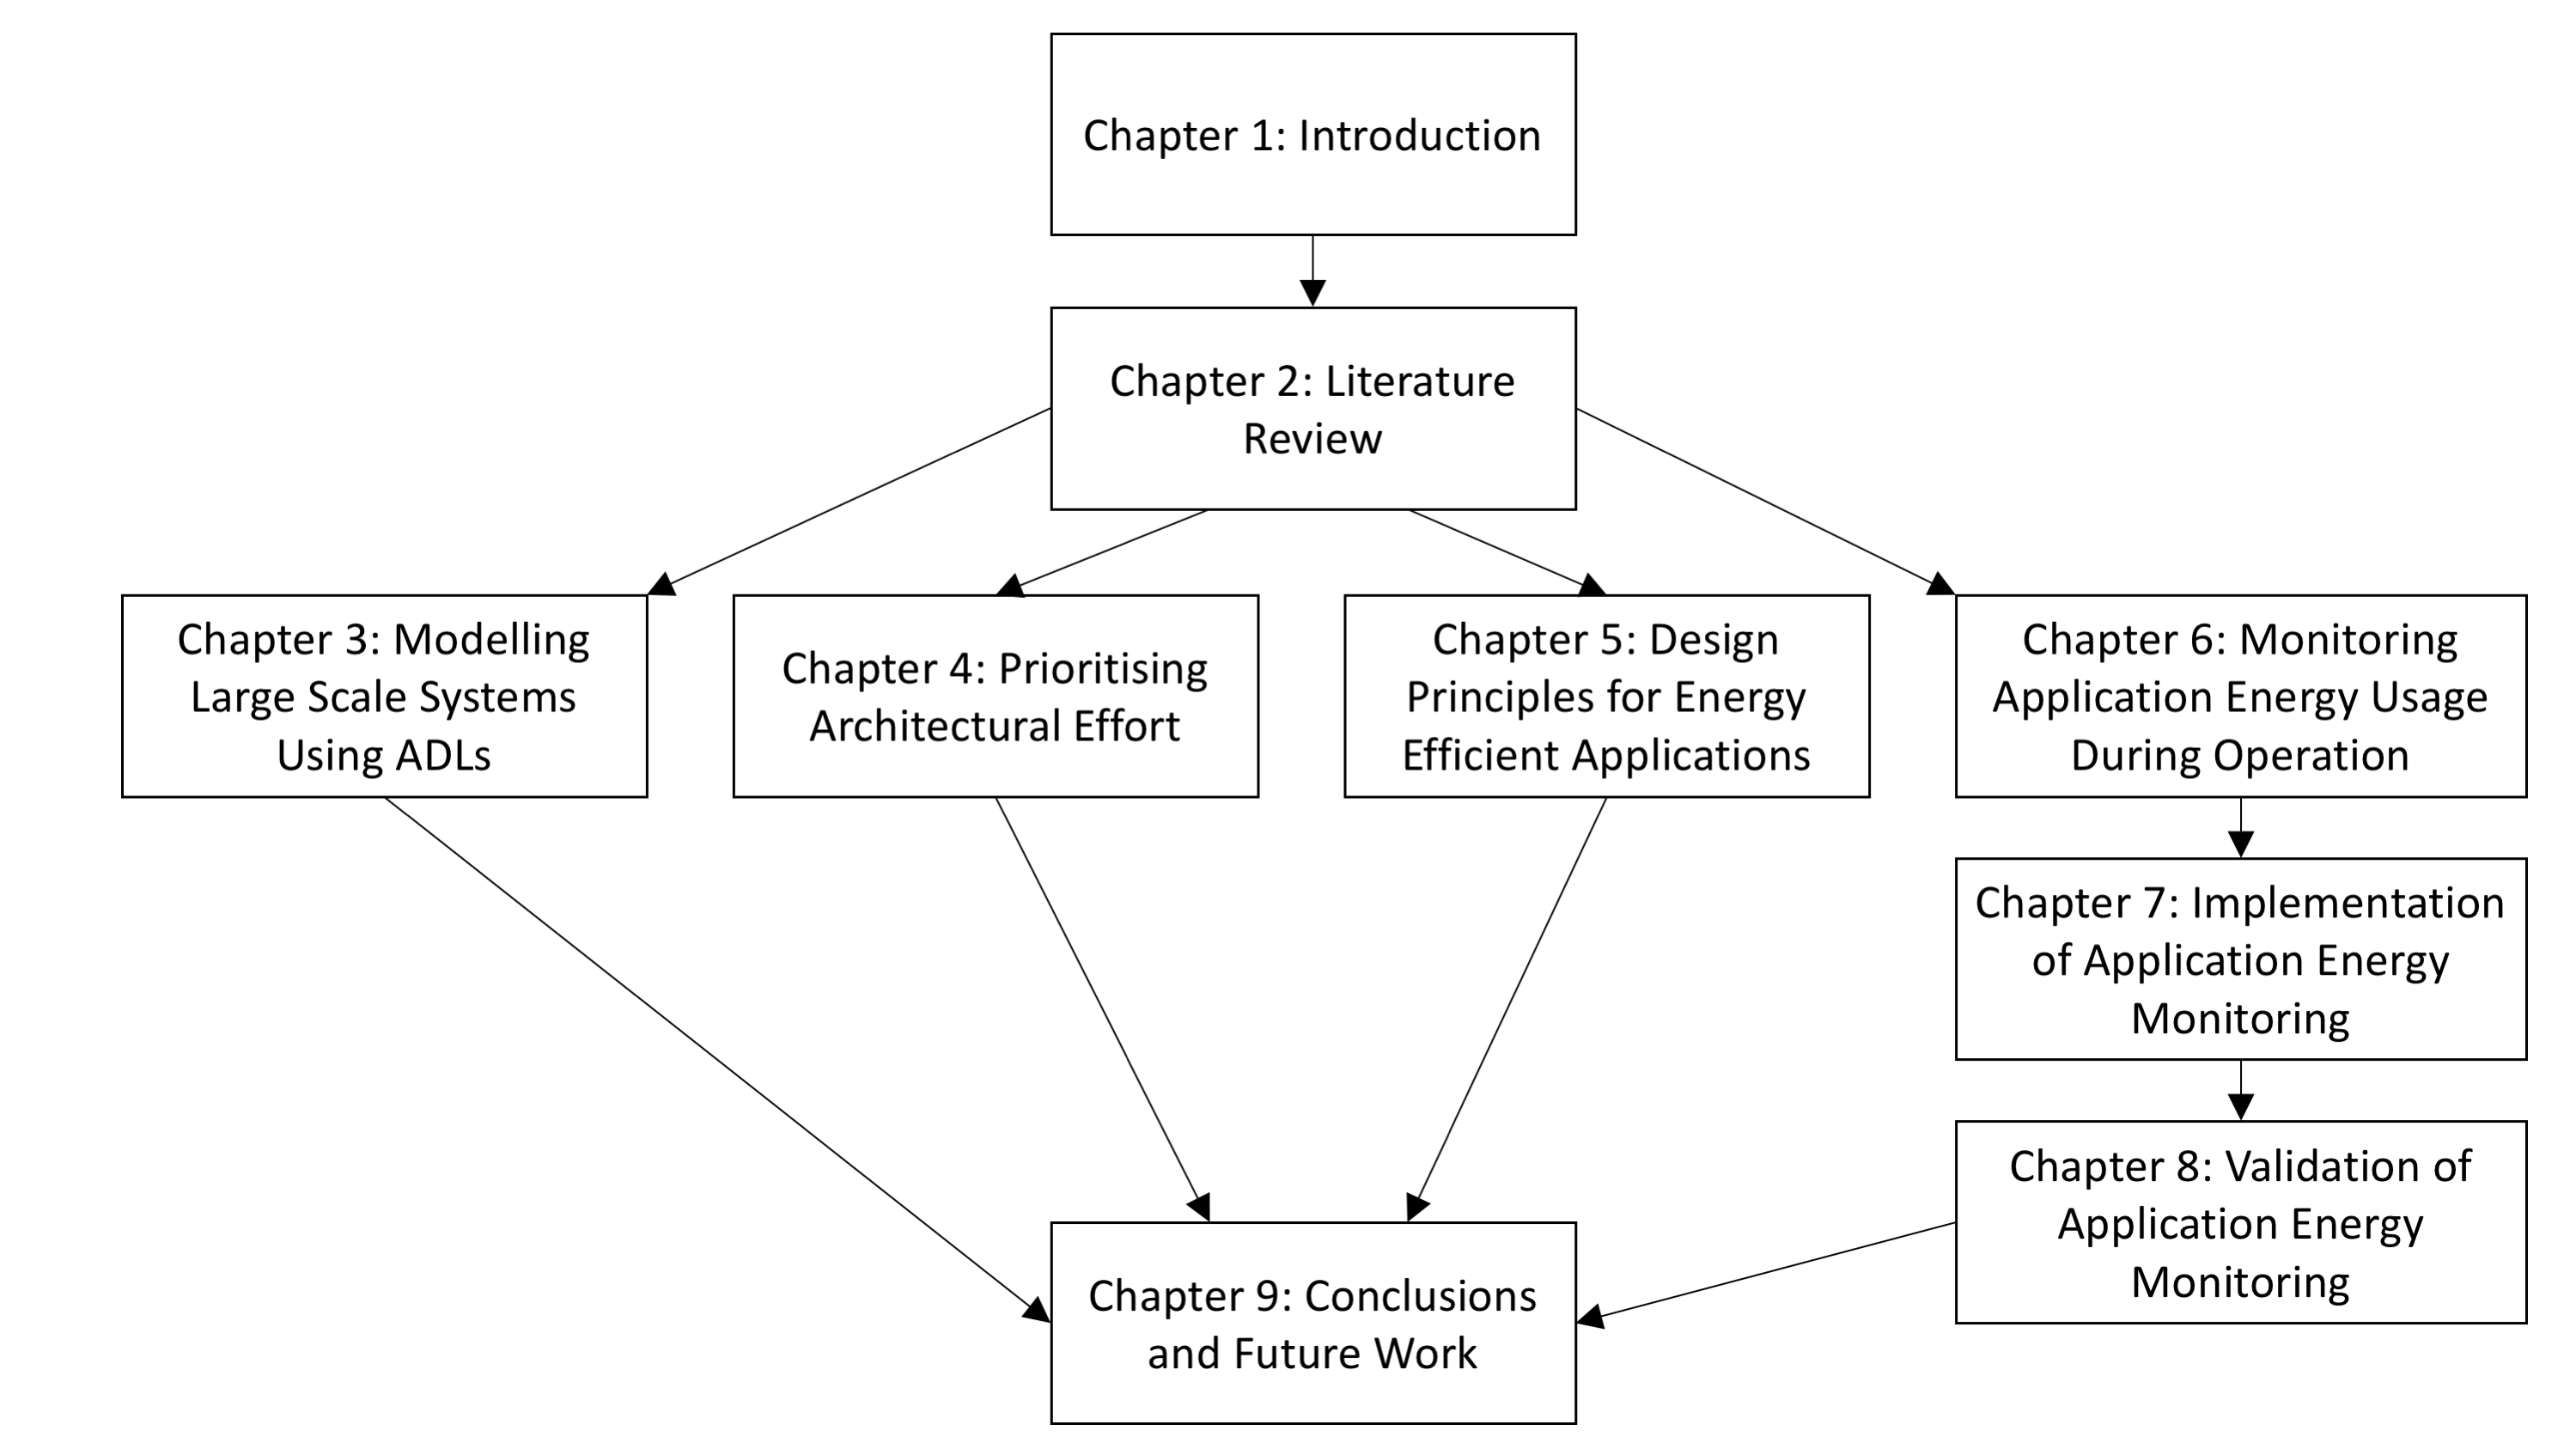
\includegraphics[width=1.0\textwidth]{Figures/intro-chapters}
\caption{Structure of the Thesis}
\label{figure:intro-chapters}
\end{figure}

\emph{Chapter 1} is this introductory chapter, setting the motivation and context for the work, defining the research questions, explaining the research approach and explaining the structure of the thesis.

\emph{Chapter 2} contains a literature review, structured into four parts, exploring the research literature in the areas of architectural description languages (ADLs), how architects should prioritise their focus for maximum effectiveness, design guidelines for energy efficiency and runtime energy consumption for IT systems.

\emph{Chapter 3} explores research question RQ1 and discusses how ADLs can be used to describe large-scale software systems and presents a significant industrial case study that explored how effective this was in practice.

\emph{Chapter 4} investigates research question RQ2 and explores the area of prioritisation of work from an architect's perspective, asking how architects prioritise their time for maximum effectiveness and presenting the results of an industrial survey into the approaches used by experienced practitioners and a validated model to guide architects, based on the insights from the survey.

\emph{Chapter 5} explores energy related design principles to answer research question RQ3 and presents a small set of heuristic design principles for designing energy-efficient software applications, derived from the experience of an industrial case study in reducing energy consumption through architectural change.

\emph{Chapter 6} addresses the fundamentals of research question RQ4 by asking how application energy usage can be monitored and estimated during the operation of a system and presents a theoretical model for solving this problem.

\emph {Chapter 7} addresses the practical aspects of research question RQ4 and presents a proof-of-concept implementation of the energy estimation model, specialised for estimating energy usage of a group of microservices processing incoming requests.

\emph{Chapter 8} validates the energy estimation approach as part of answering research question RQ4 and presents the work performed to validate the energy estimation technology. This involved running a number of carefully controlled test scenarios and using the tool to estimate their energy usage, while also deriving the same estimation through a separate, independent technique, using these secondary estimations to validate the outputs of the model and the tool.

\emph {Chapter 9} summarises the research work, draws conclusions from it to answer the research questions and discusses possible future research work in each area.



